\documentclass[abstract=on,10pt,a4paper,bibliography=totocnumbered]{article}
\usepackage[paper=a4paper,left=35mm,right=35mm,top=25mm,bottom=30mm]{geometry}
\usepackage[doublespacing]{setspace}
\usepackage[english]{babel}
\usepackage[utf8]{inputenc}
\usepackage[round]{natbib}
\usepackage{amsmath}
\usepackage{colortbl}
\usepackage{amsfonts}
\usepackage{amssymb}
\usepackage{gensymb}
\usepackage{graphicx}
\usepackage{tikz}
\usepackage{enumerate}
\usepackage{enumitem}
\usepackage{subcaption}
\usepackage{booktabs}
\usepackage[hidelinks]{hyperref}
\usepackage[nameinlink]{cleveref}
\usepackage{lineno}
\usepackage{multirow}
\usepackage{arydshln}
\usepackage[flushleft]{threeparttable}
\usepackage[colorinlistoftodos]{todonotes}
\usepackage{scalerel}
\usepackage{tikz}
\usetikzlibrary{svg.path}

%------------------------------------------------------------------------------
%	Some Styling
%------------------------------------------------------------------------------
% Creating some TikZ styles
\tikzset{
  nonterminal/.style = {rectangle
    , minimum size = 6mm
    , very thick
    , draw = black!
  }
}

% Changing the style of captions in figures etc.
\captionsetup{labelfont=bf, format=plain, font=small}

% For supplementary material
\newcommand{\beginappendix}{%
  \setcounter{table}{0}
  \renewcommand{\thetable}{S\arabic{table}}%
  \setcounter{figure}{0}
  \renewcommand{\thefigure}{S\arabic{figure}}%
  \setcounter{equation}{0}
  \renewcommand{\theequation}{Equation S\arabic{equation}}%
  \setcounter{section}{0}
  \renewcommand{\thesection}{A.\arabic{section}}%
}

% Change how equations are referenced
\renewcommand{\theequation}{Equation \arabic{equation}}%

% To be able to put an ORCID
\definecolor{orcidlogocol}{HTML}{A6CE39}
\tikzset{
  orcidlogo/.pic={
    \fill[orcidlogocol] svg{M256,128c0,70.7-57.3,128-128,128C57.3,256,0,198.7,0,128C0,57.3,57.3,0,128,0C198.7,0,256,57.3,256,128z};
    \fill[white] svg{M86.3,186.2H70.9V79.1h15.4v48.4V186.2z}
                 svg{M108.9,79.1h41.6c39.6,0,57,28.3,57,53.6c0,27.5-21.5,53.6-56.8,53.6h-41.8V79.1z M124.3,172.4h24.5c34.9,0,42.9-26.5,42.9-39.7c0-21.5-13.7-39.7-43.7-39.7h-23.7V172.4z}
                 svg{M88.7,56.8c0,5.5-4.5,10.1-10.1,10.1c-5.6,0-10.1-4.6-10.1-10.1c0-5.6,4.5-10.1,10.1-10.1C84.2,46.7,88.7,51.3,88.7,56.8z};
  }
}
\newcommand\orcid[1]{\href{https://orcid.org/#1}{\mbox{\scalerel*{

\begin{tikzpicture}[yscale=-1,transform shape]
  \pic{orcidlogo};
\end{tikzpicture}
}{|}}}}

%------------------------------------------------------------------------------
%	Titlepage: Header
%------------------------------------------------------------------------------
\title{\textbf{Appendix}\\ Flooding of the Okavango Delta influences
Connectivity for Dispersing African Wild Dogs}

% List of Authors
\author{
  David D. Hofmann\textsuperscript{1,2,\S} \orcid{0000-0003-3477-4365} \and
  Dominik M. Behr\textsuperscript{1,2} \orcid{0000-0001-7378-8538} \and
  John W. McNutt\textsuperscript{2} \and
  Arpat Ozgul\textsuperscript{1} \orcid{0000-0001-7477-2642} \and
  Gabriele Cozzi\textsuperscript{1,2} \orcid{0000-0002-1744-1940}
}

% Reduce spacing between authors
\makeatletter
\def\and{%
  \end{tabular}%
  \hskip -0.5em \@plus.17fil\relax
  \begin{tabular}[t]{c}}
\makeatother

% Current Date
% \date{\today}

% And here the masterpiece begins
\begin{document}

% Change page numbering
\pagenumbering{gobble}

% Required to be able to cite
\bibliographystyle{apalike}

% Create Titlepage
\maketitle

%------------------------------------------------------------------------------
%	Titlepage: Additional Info
%------------------------------------------------------------------------------
\begin{flushleft}

\vspace{0.5cm}

\textsuperscript{1} Department of Evolutionary Biology and Environmental
Studies, University of Zurich, Winterthurerstarsse 190, 8057 Zurich,
Switzerland.

\textsuperscript{2} Botswana Predator Conservation Program, Private Bag 13,
Maun, Botswana.

\textsuperscript{\S} Corresponding author (david.hofmann2@uzh.ch)

\vspace{4cm}

\textbf{Running Title:} Seasonal Flooding of the Okavango Delta and its
Consequences for African Wild Dog Dispersal and Connectivity

\vspace{0.5cm}

\textbf{Keywords:} movement, connectivity, seasonality, dispersal, conservation,
permeability

\end{flushleft}

%------------------------------------------------------------------------------
%	Main Text
%------------------------------------------------------------------------------
\newpage

% Change page numbering
\pagenumbering{arabic}

% Create linenumbers
% \linenumbers

% Change to appendix counters
\appendix
\beginappendix

%------------------------------------------------------------------------------
%  Appendix S1: Difference Heatmap
%------------------------------------------------------------------------------
\newpage
\section{Difference Heatmap}
\begin{figure}[htbp]
  \begin{center}
  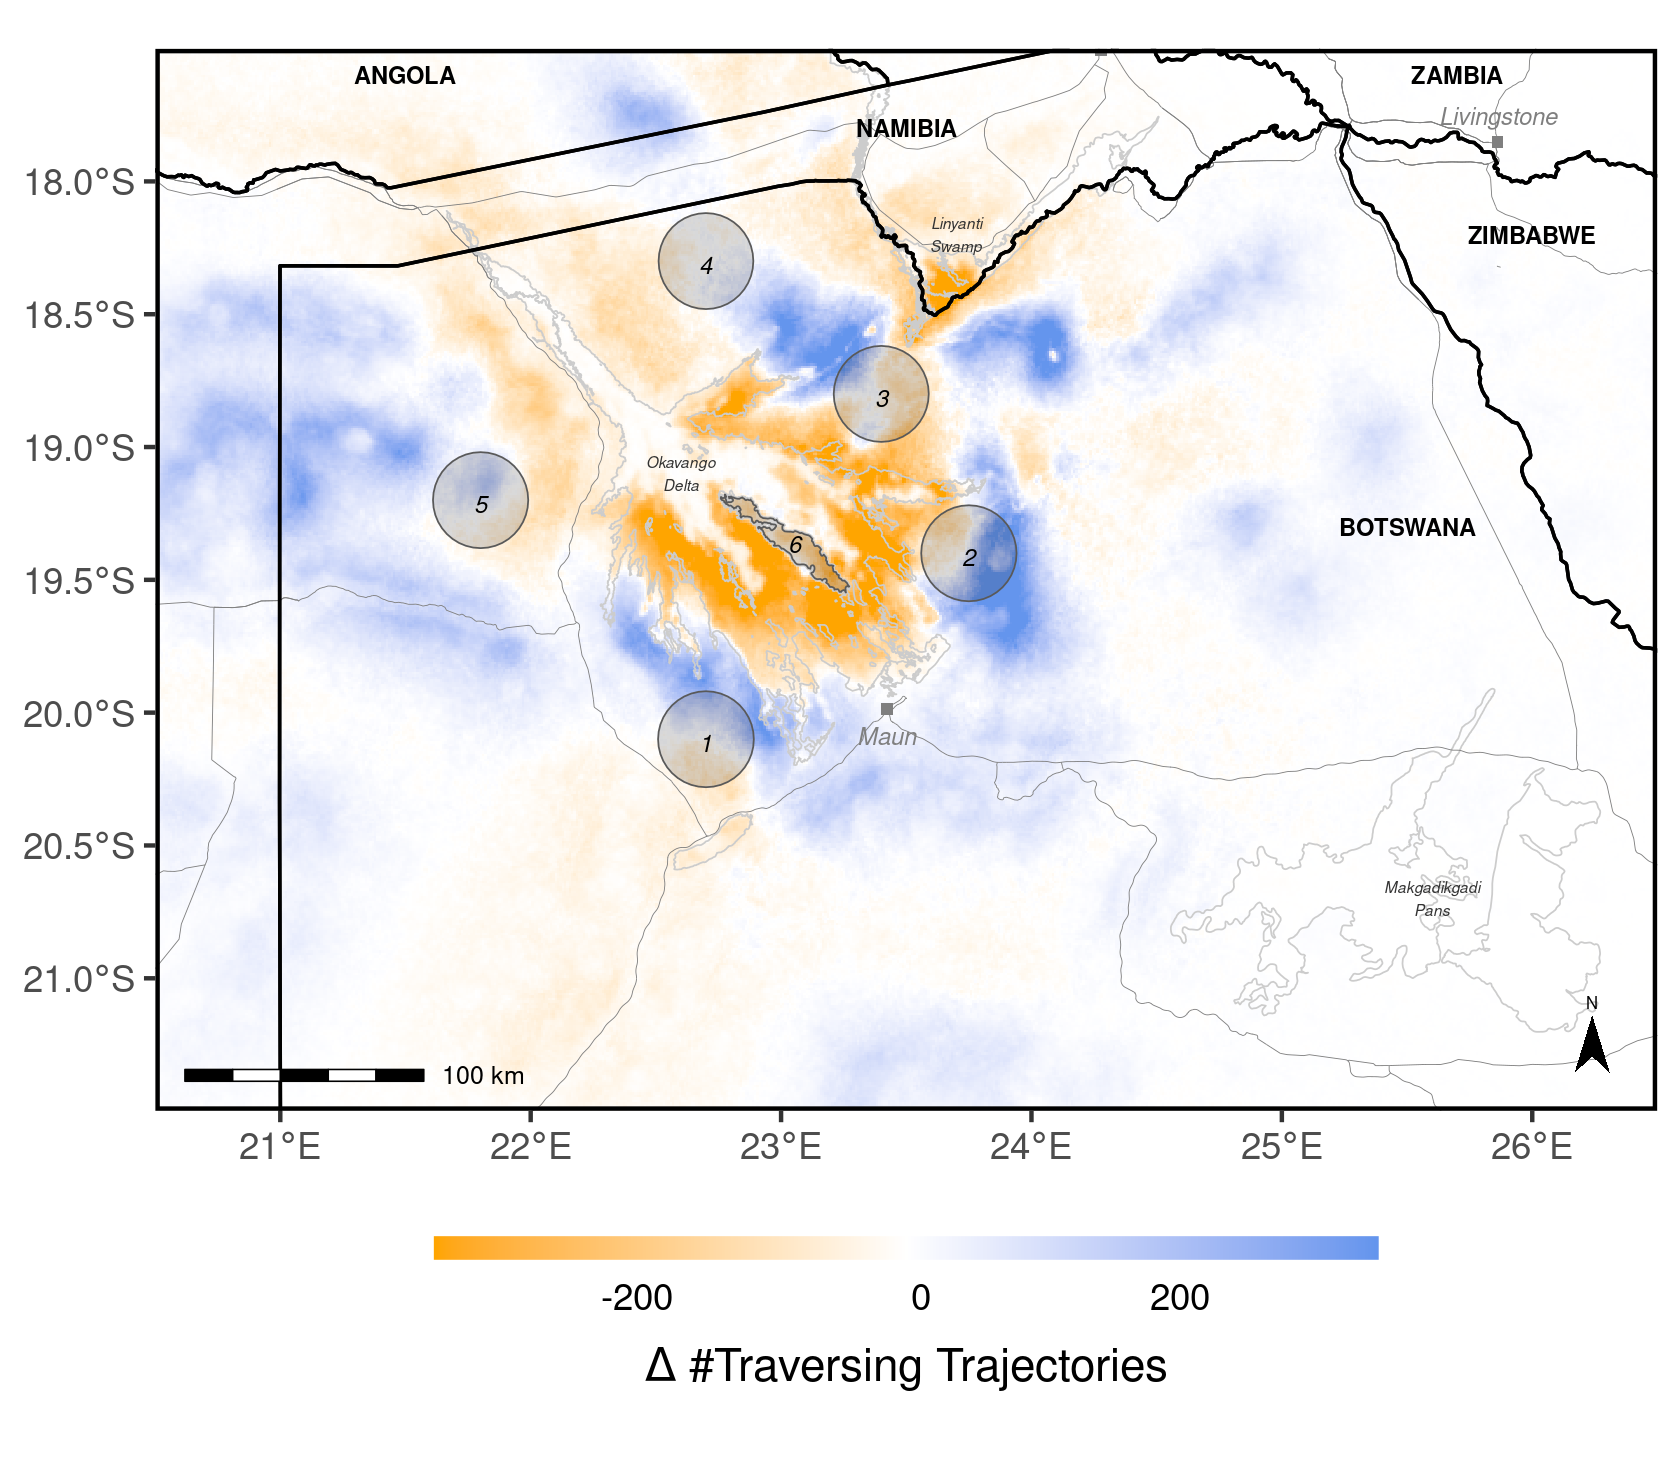
\includegraphics[width = \textwidth]{99_HeatmapsDifference.png}
  \caption{}
  \label{HeatmapsDifference}
  \end{center}
\end{figure}

%------------------------------------------------------------------------------
%  Appendix S2: Source-Specific Heatmaps
%------------------------------------------------------------------------------
\newpage
\section{Source-Specific Heatmaps}
\begin{figure}[htbp]
  \begin{center}
  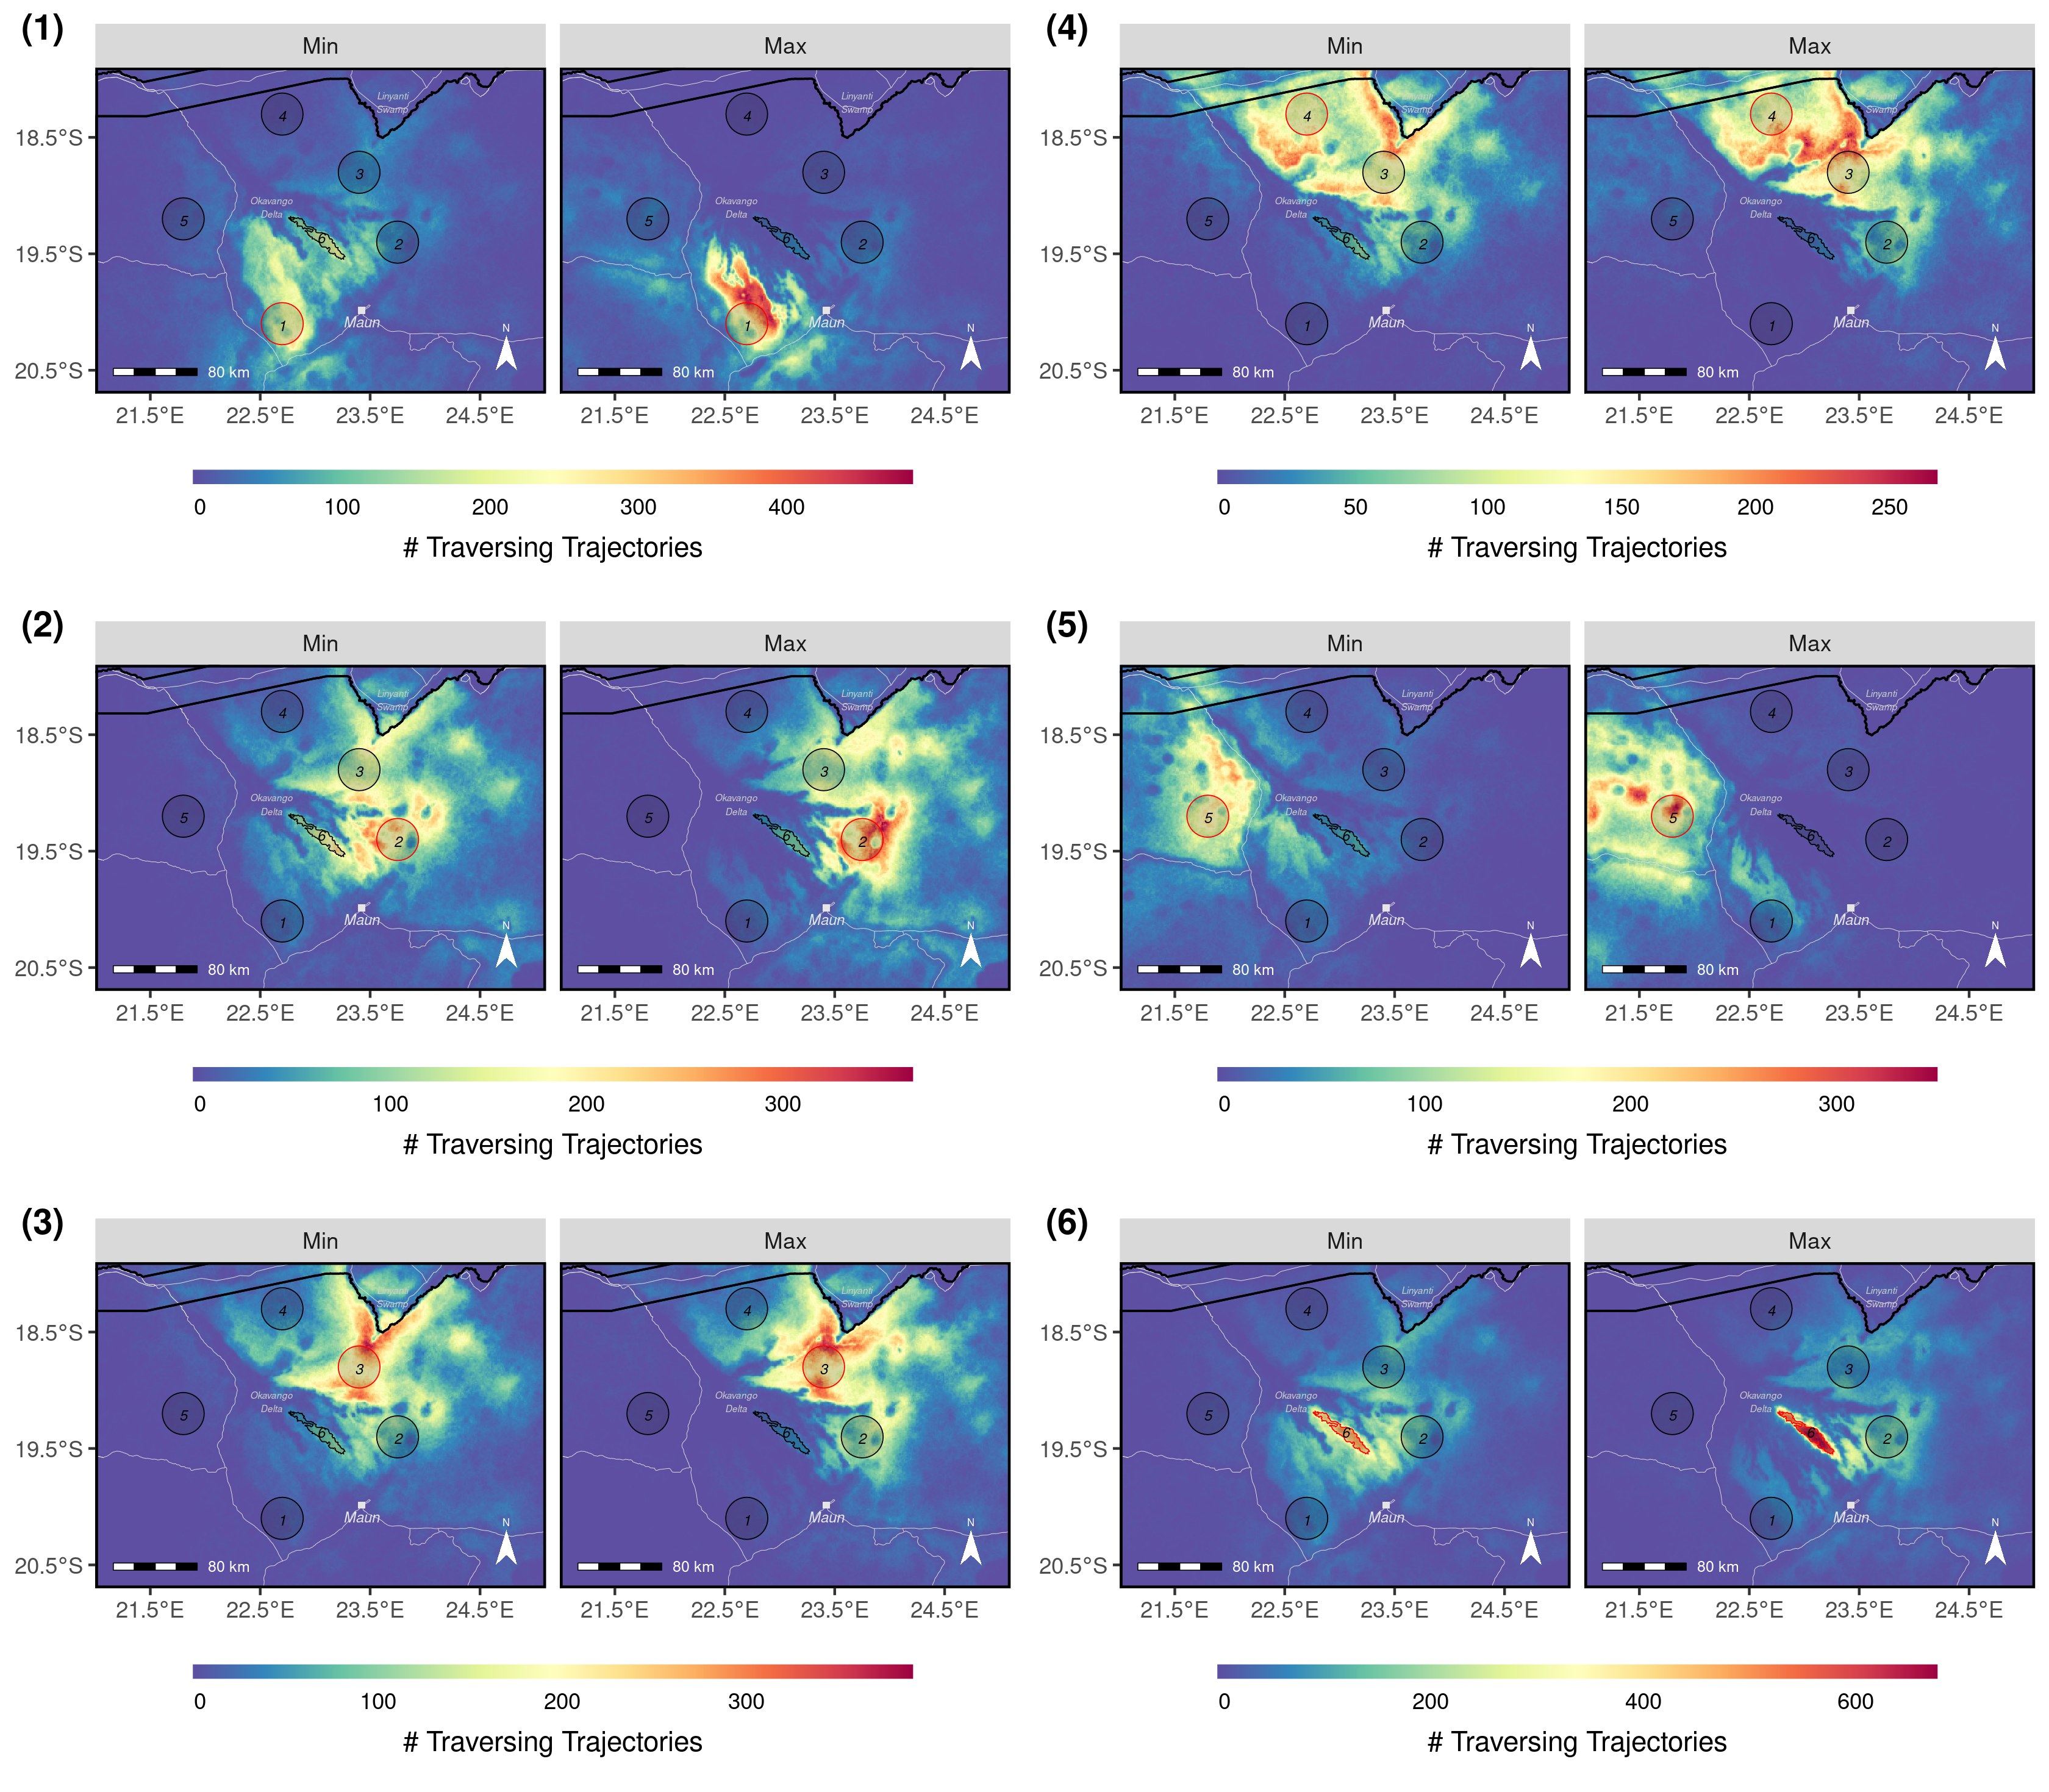
\includegraphics[width = \textwidth]{99_HeatmapsIndividual.png}
  \caption{}
  \label{Heatmaps}
  \end{center}
\end{figure}

%------------------------------------------------------------------------------
%  Appendix S3: Difference Betweenness
%------------------------------------------------------------------------------
\newpage
\section{Difference Betweenness}
\begin{figure}[htbp]
  \begin{center}
  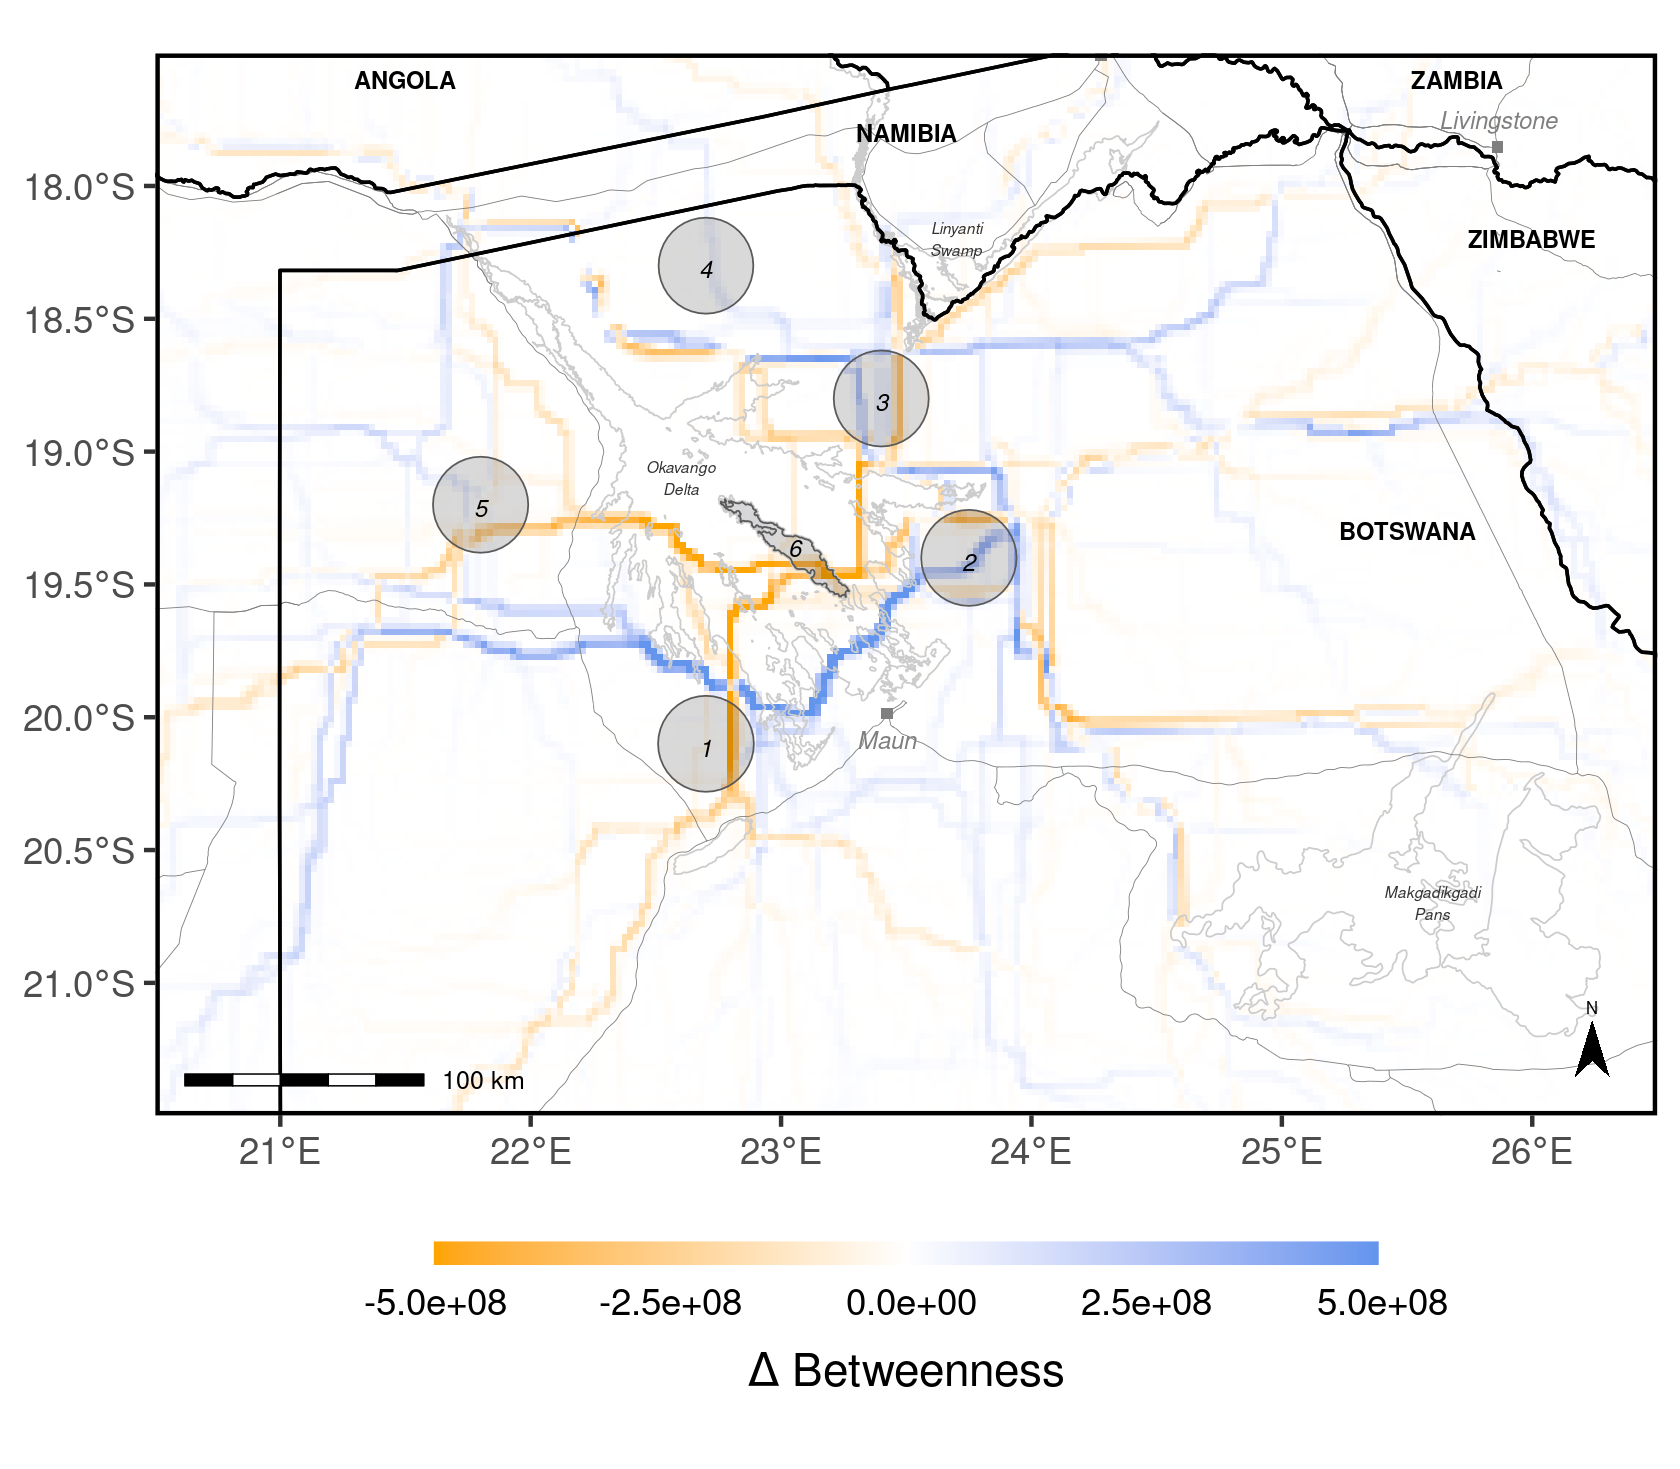
\includegraphics[width = \textwidth]{99_BetweennessDifference.png}
  \caption{}
  \label{BetweennessDifference}
  \end{center}
\end{figure}

%------------------------------------------------------------------------------
%  Appendix S4: Source-Specific Betweenness
%------------------------------------------------------------------------------
\newpage
\section{Source-Specific Betweenness}
\begin{figure}[htbp]
  \begin{center}
  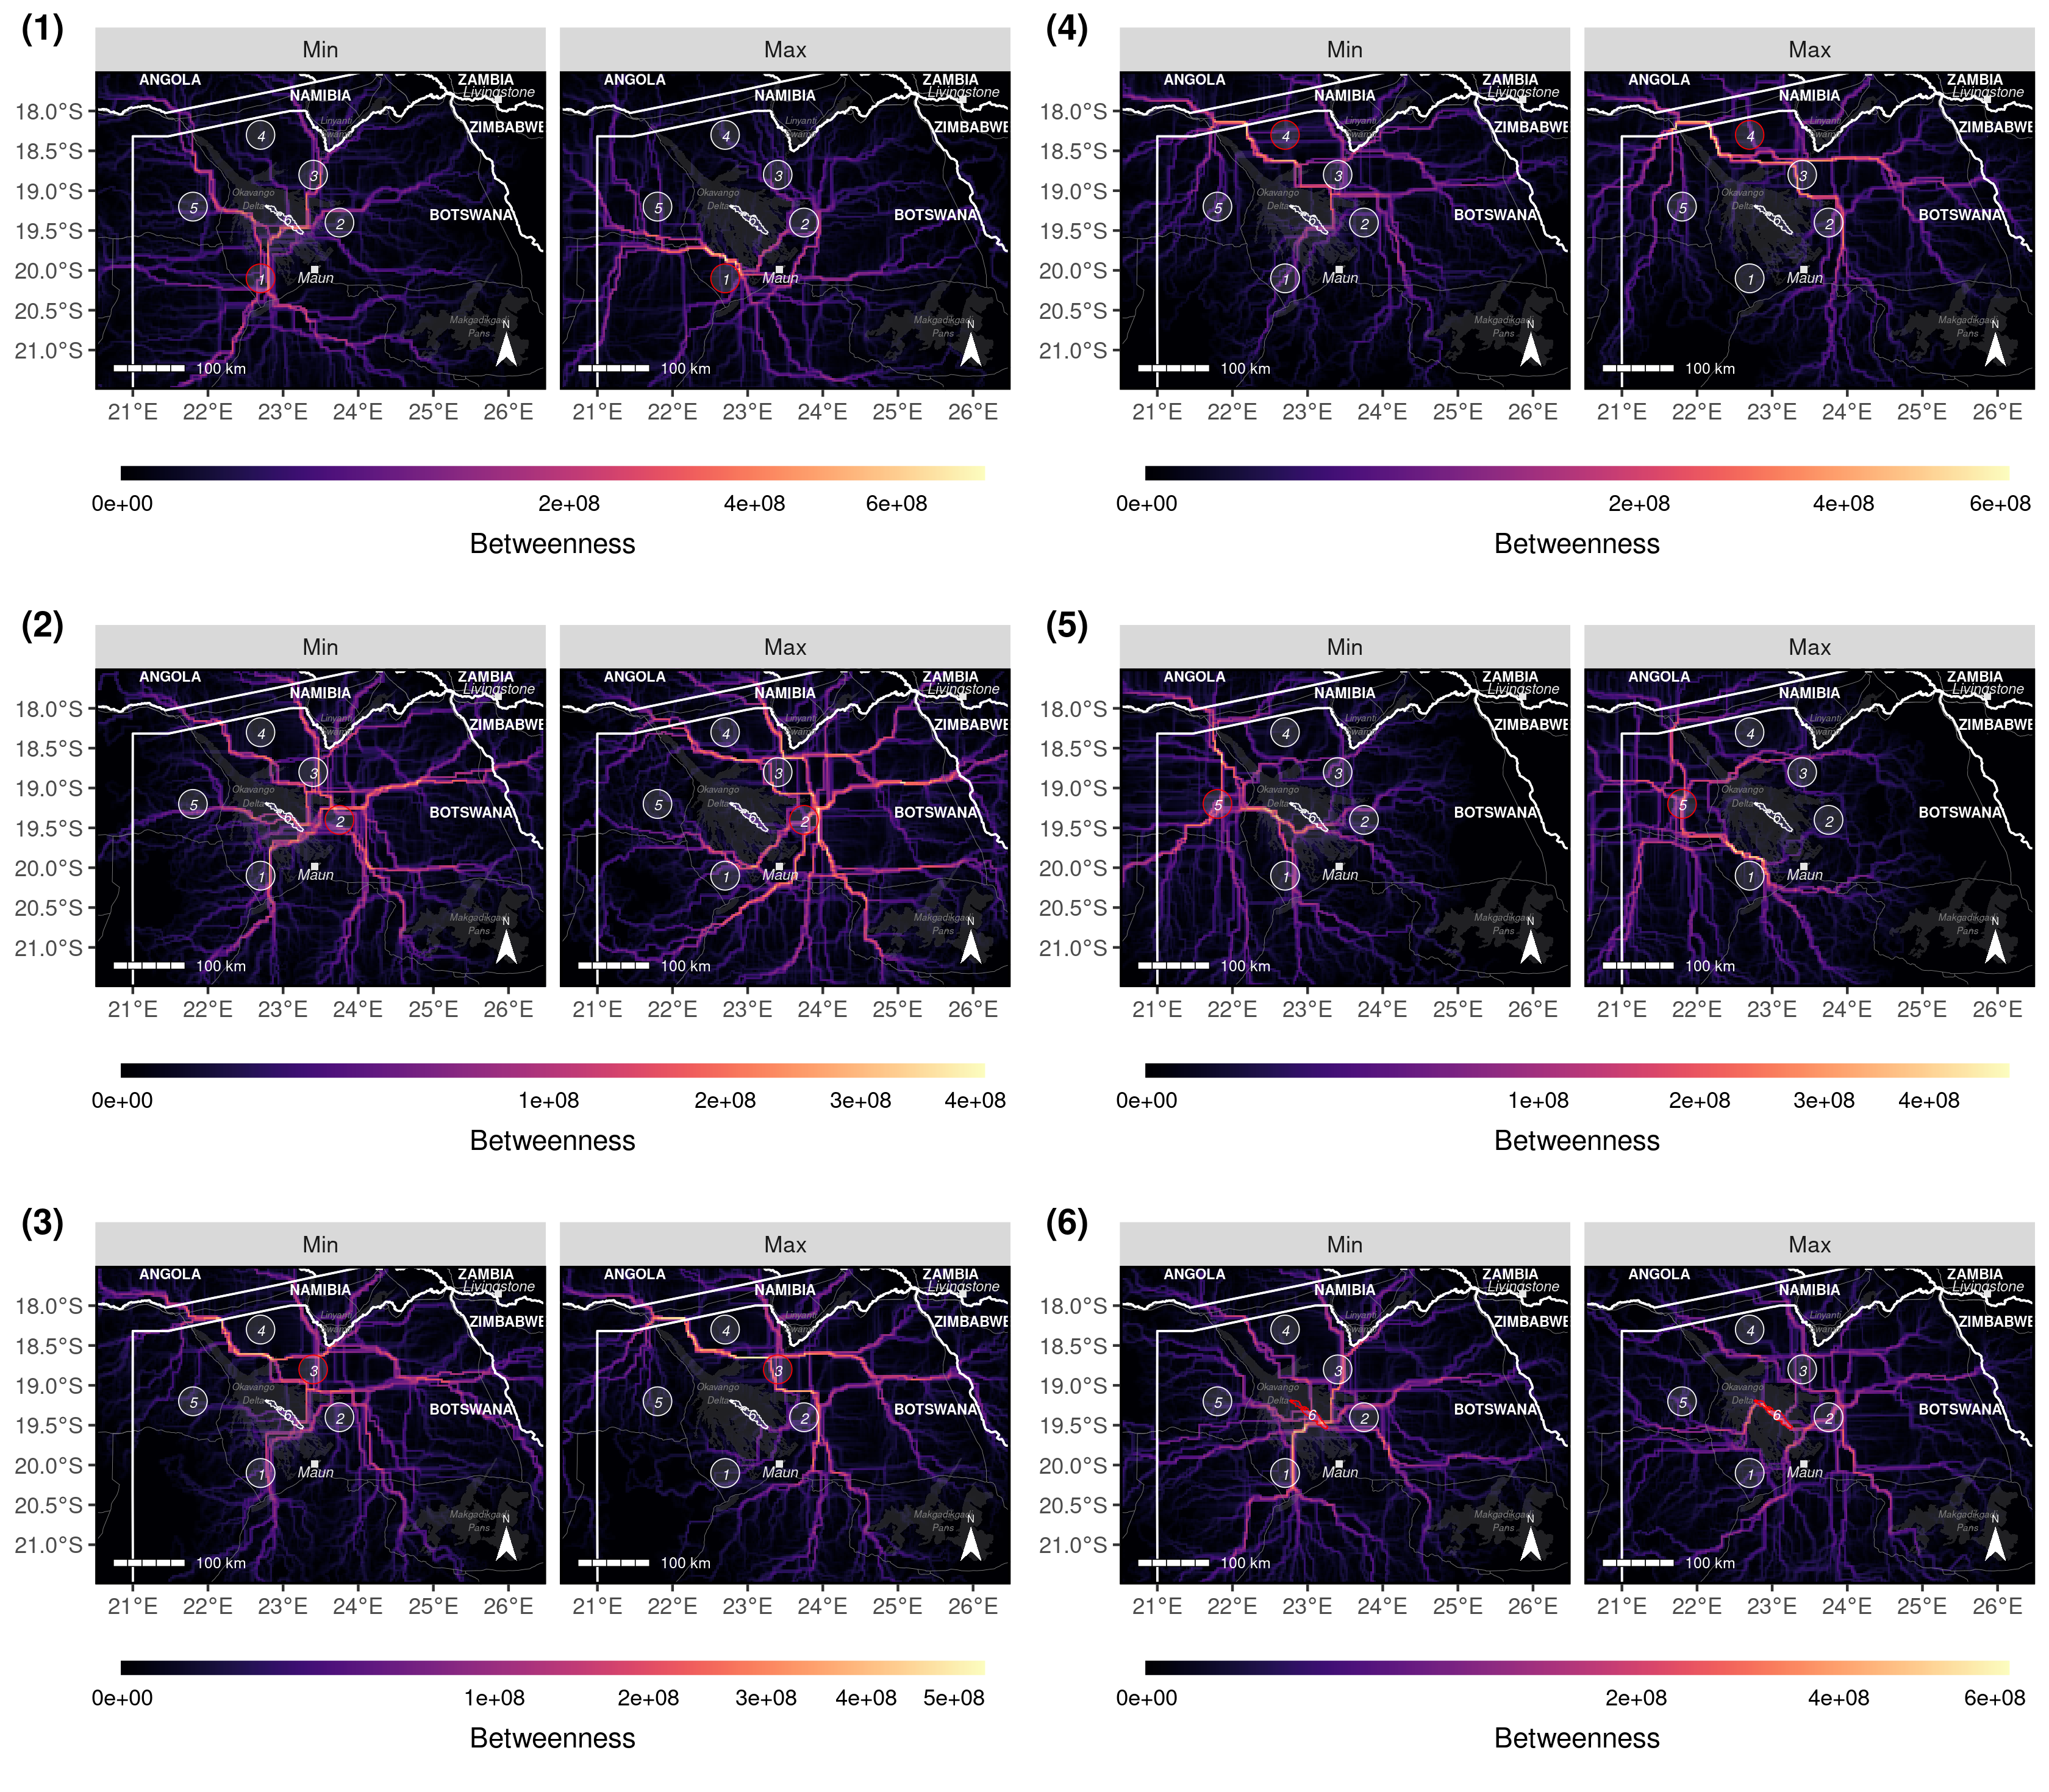
\includegraphics[width = \textwidth]{99_BetweennessIndividual.png}
  \caption{}
  \label{Betweenness}
  \end{center}
\end{figure}

%------------------------------------------------------------------------------
%  Appendix S5: Source-Specific Betweenness
%------------------------------------------------------------------------------
\newpage
\section{Source-Specific Inter-Patch Connectivity}
\begin{figure}[htbp]
  \begin{center}
  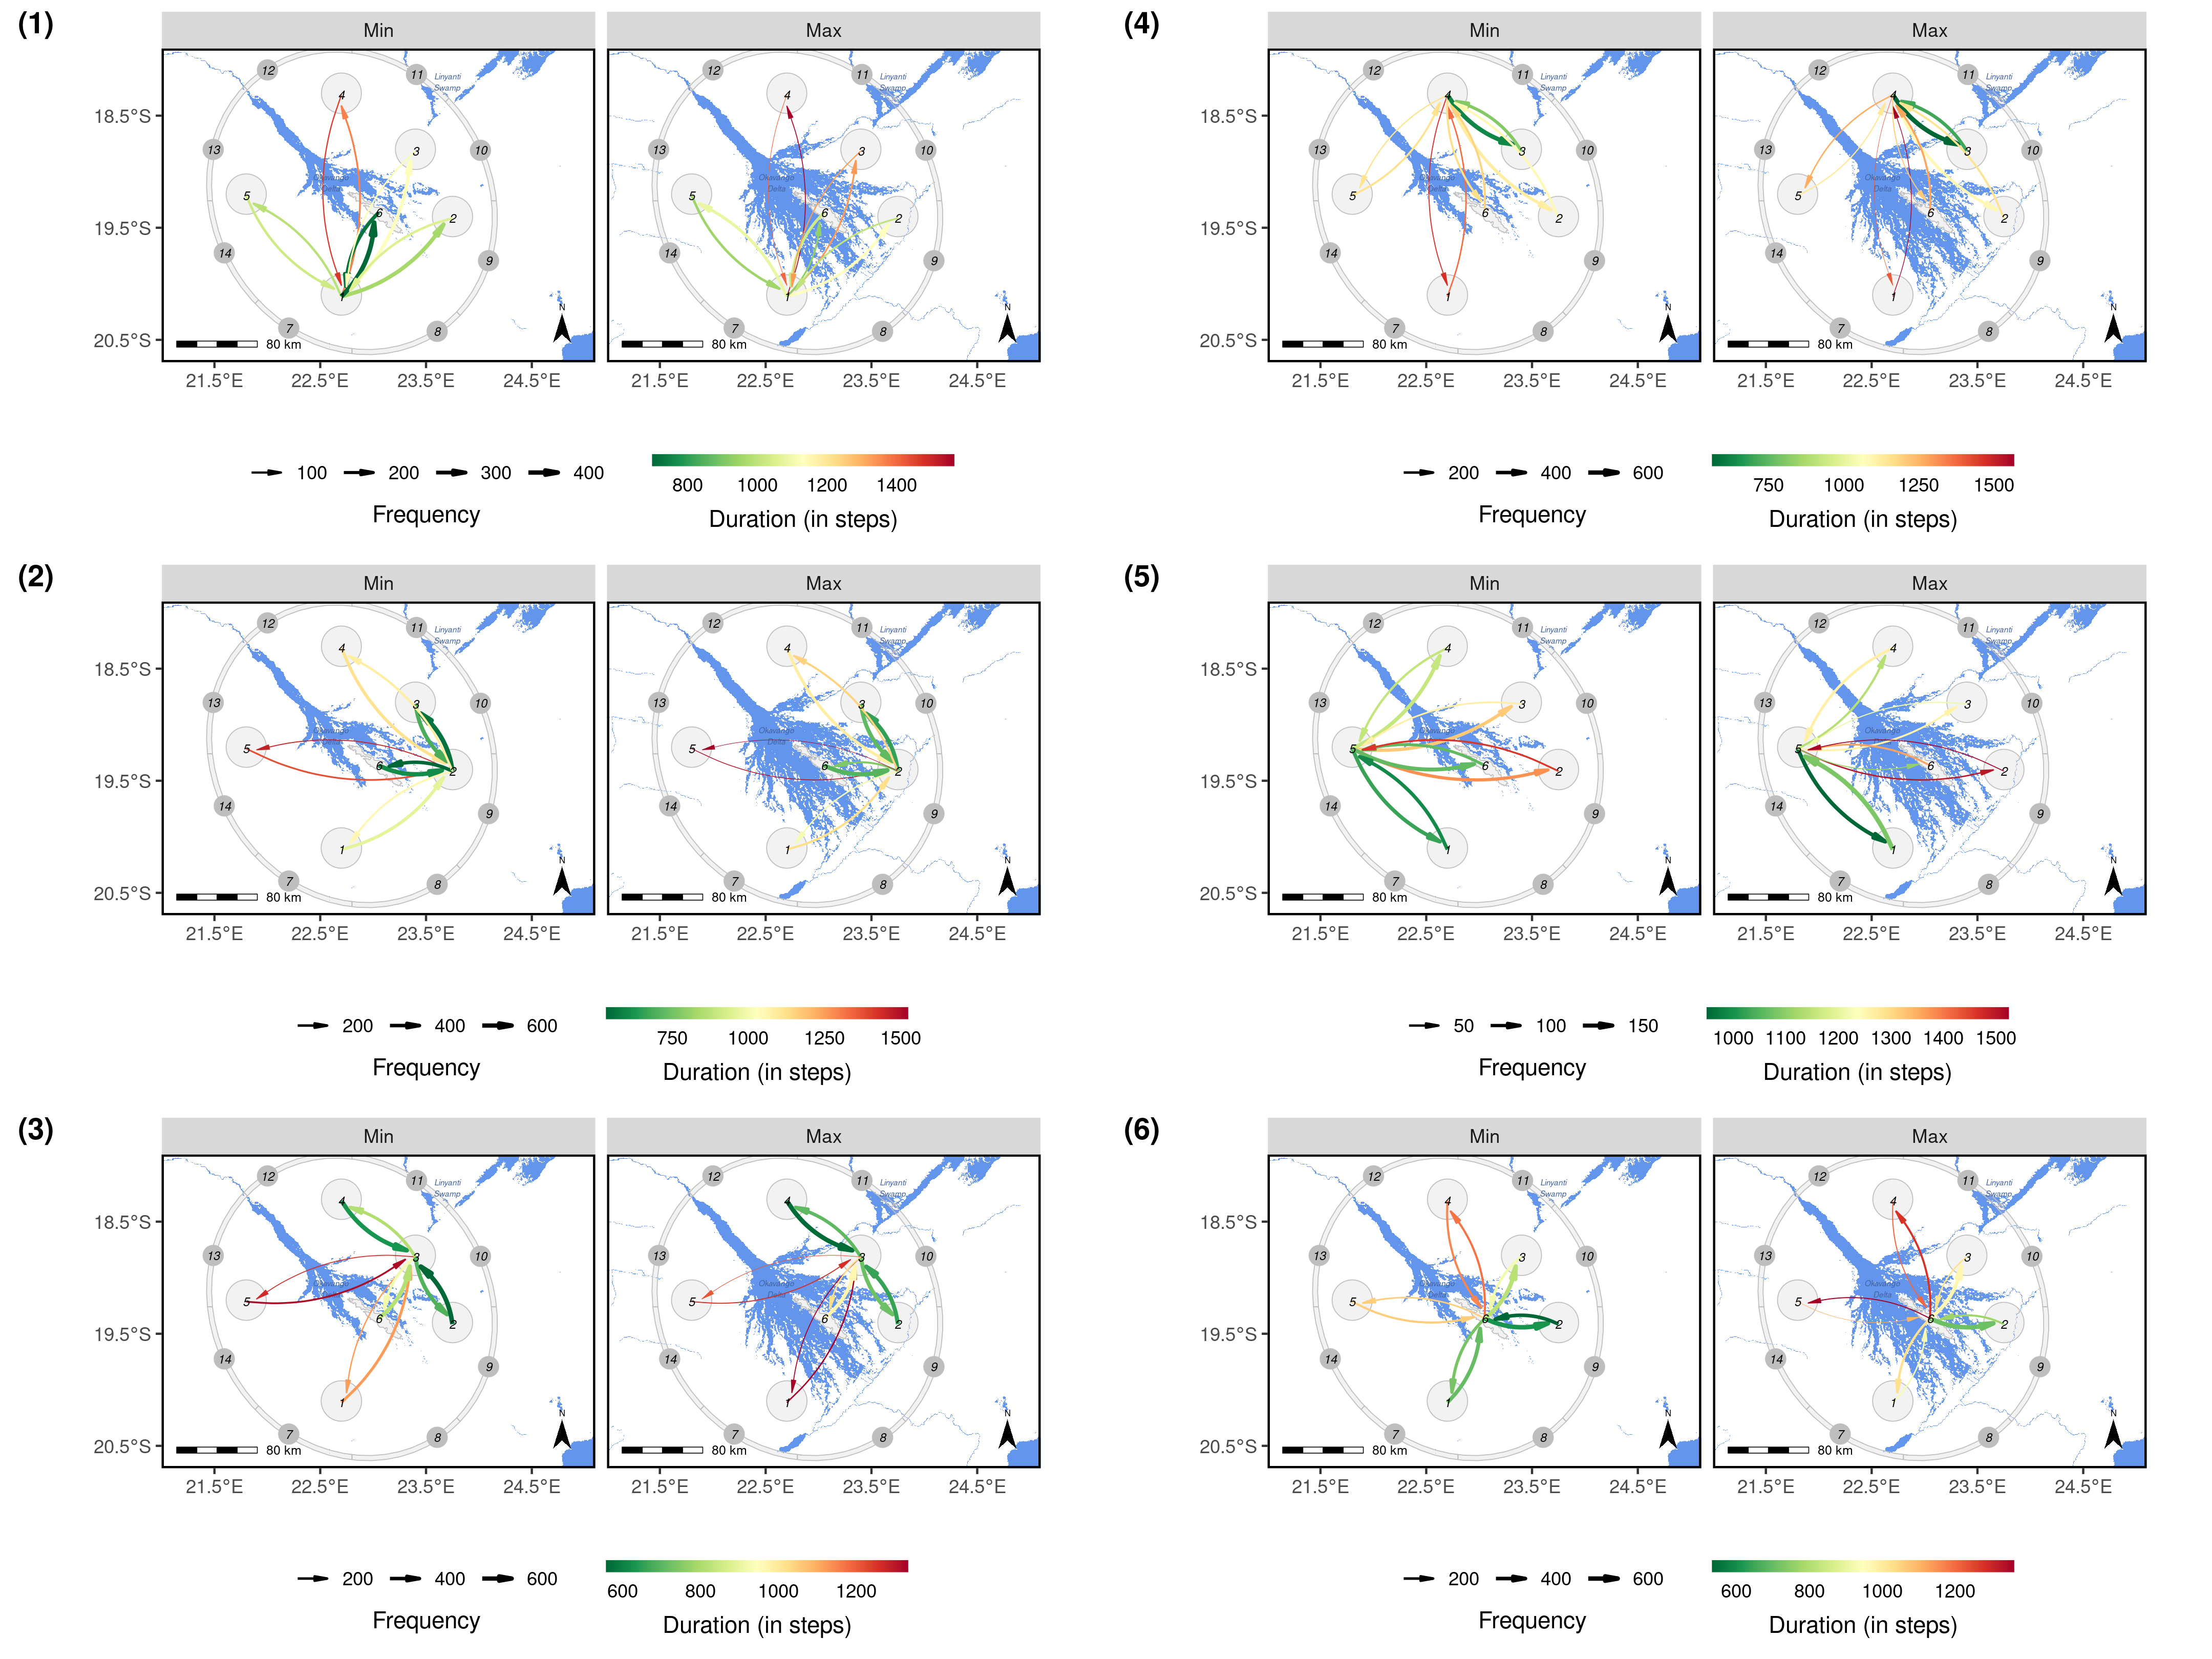
\includegraphics[width = \textwidth]{99_IPCMain.png}
  \caption{}
  \label{IPCMain}
  \end{center}
\end{figure}

\begin{figure}[htbp]
  \begin{center}
  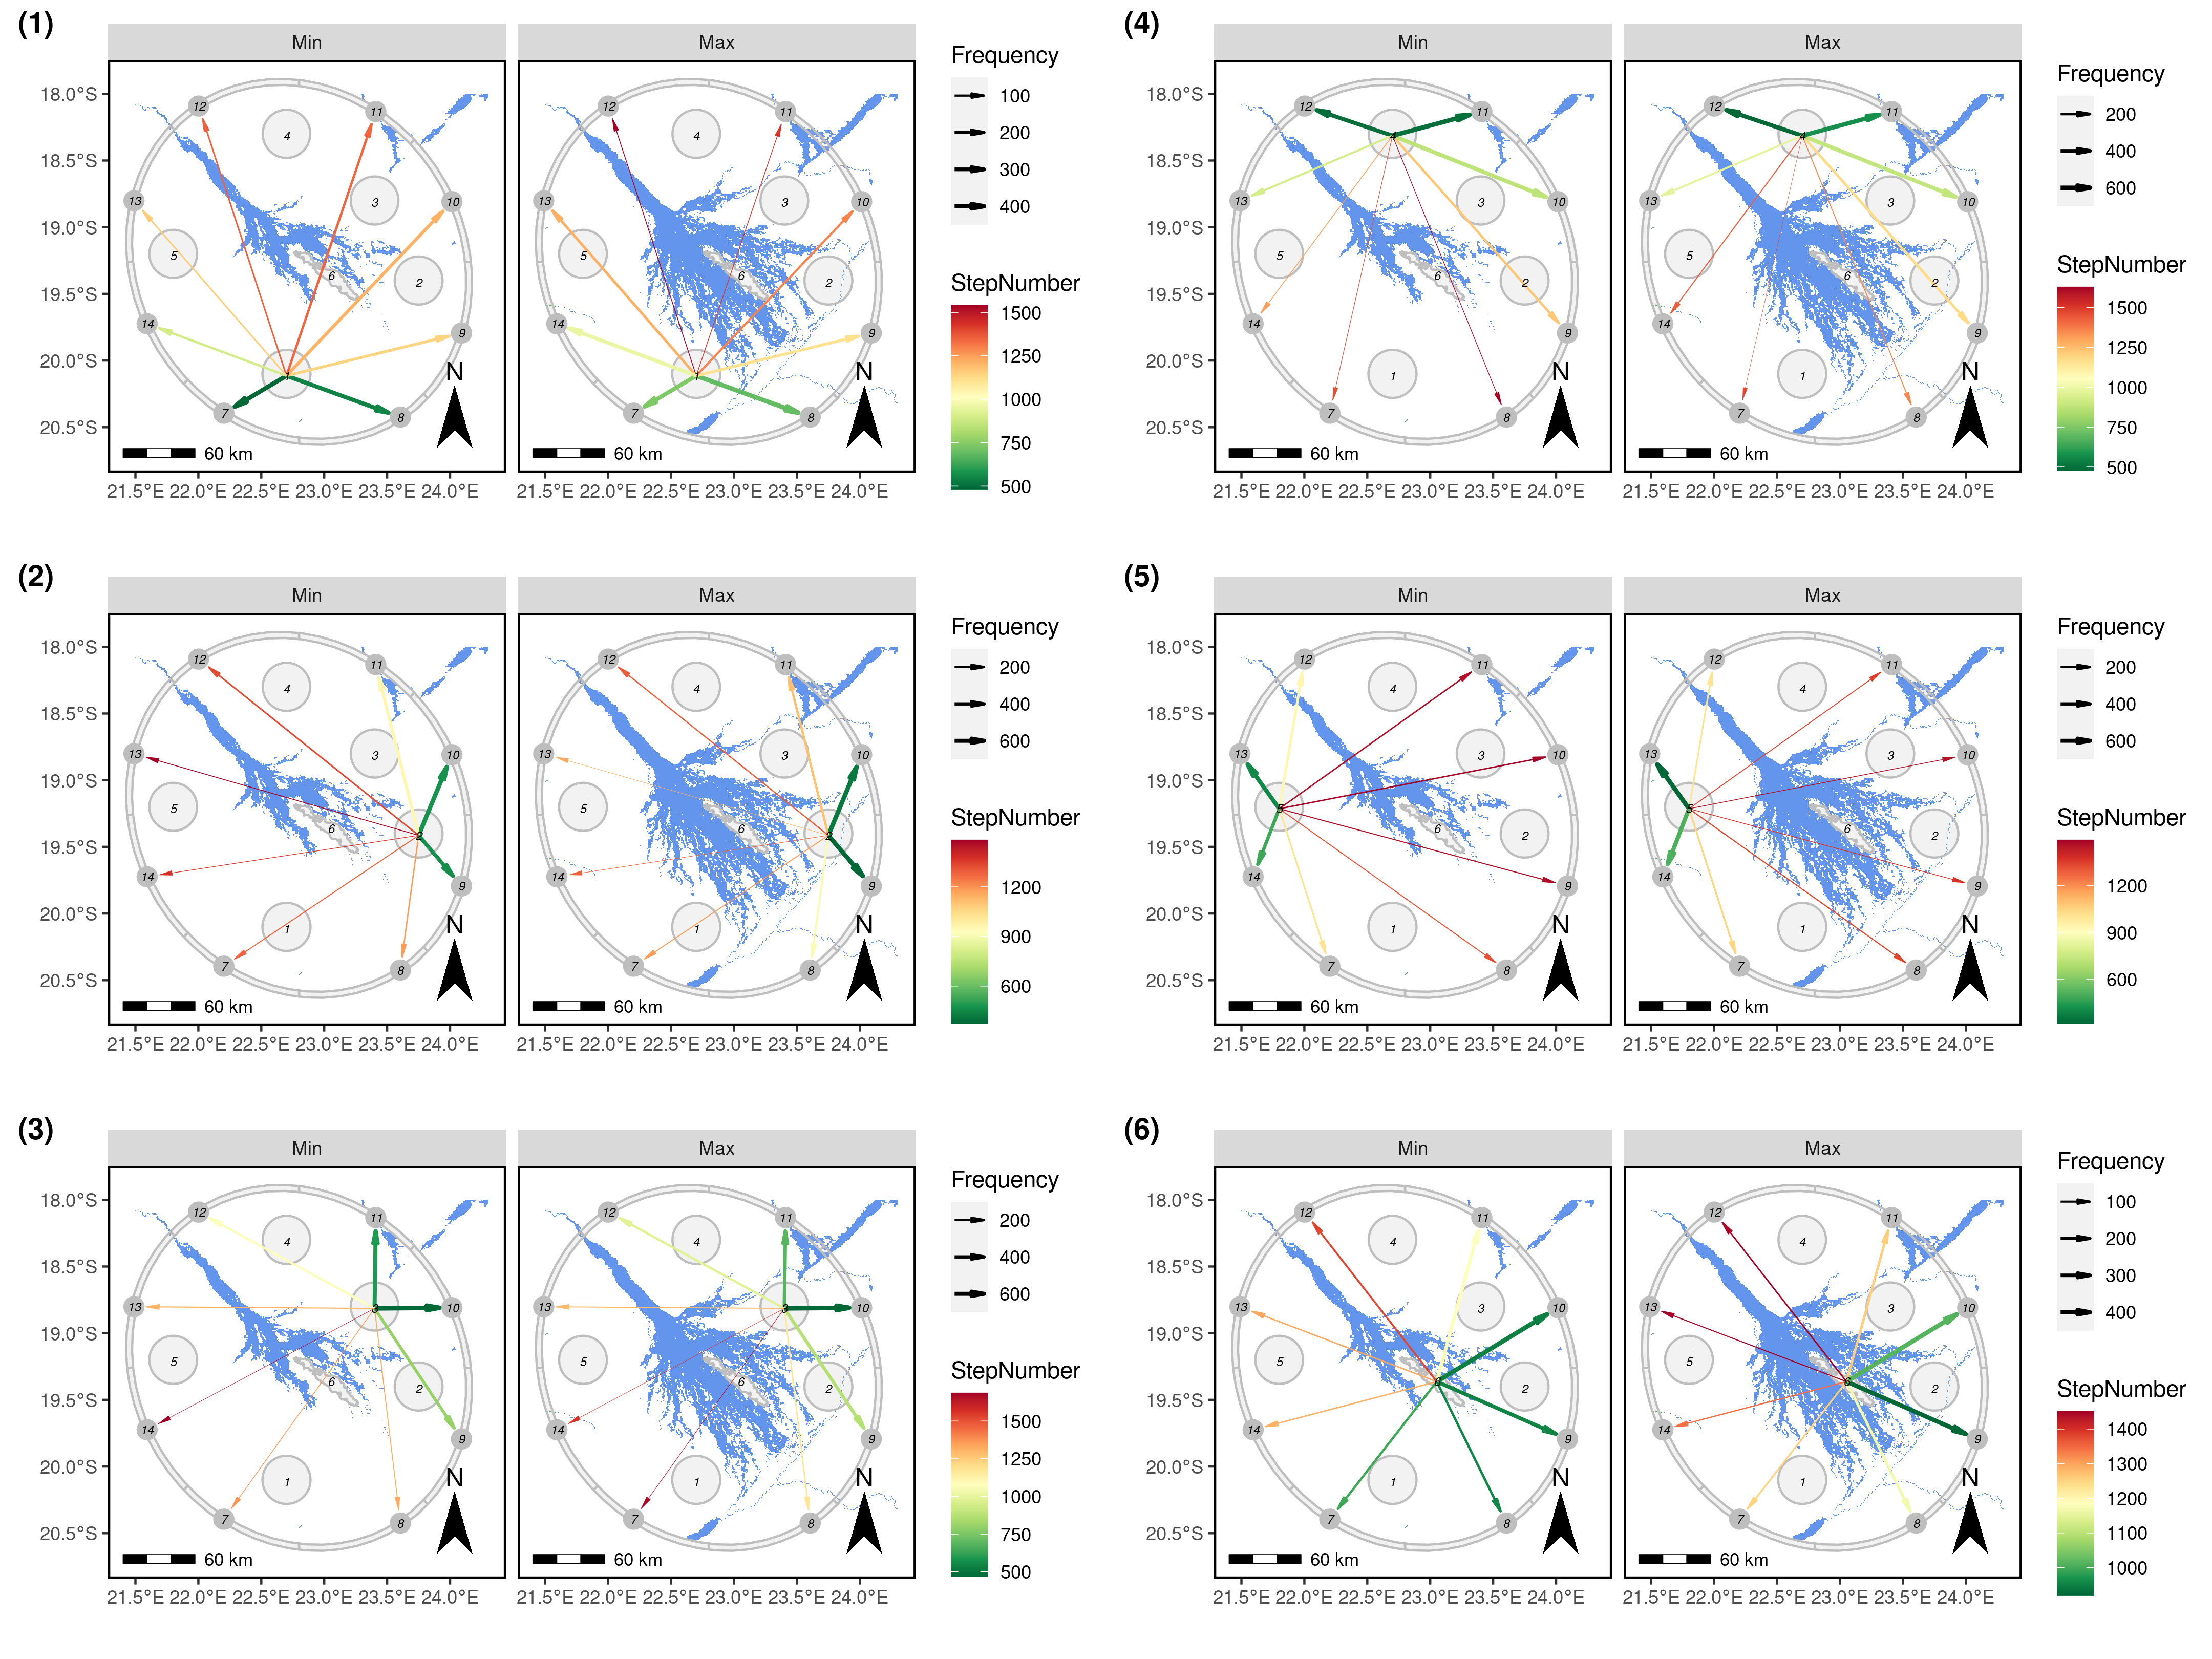
\includegraphics[width = \textwidth]{99_IPCBuffer.png}
  \caption{}
  \label{IPCBuffer}
  \end{center}
\end{figure}


\newpage
\begingroup
\singlespacing
\bibliography{Literatur}
\endgroup

\end{document}
